% arara: xelatex: {synctex: true}
% arara: indent: {overwrite: yes}
\documentclass[]{IMTexam}

\usepackage{IMTtikz}

\givecredits
\author{Isabella B.}
\USPN{11810773}
\date{}
\lecture{Física I} % disciplina
\lcode{4302111}
\hwtype{Resolução} % o que é
\examname{Lista 7} % prova

\begin{document}

\maketitle

\begin{questions}

	\question Considere um triângulo equilátero, da lado $ L $ e densidade superficial de massa $ \sigma = \sigma_0 $ constante. Calcule a posição do centro de massa.

	\begin{solution}
		Sendo o centro de massa dado por
		\begin{equation}\label{eq:Cmass}
			\vec{R}=\dfrac{1}{M}\int_{V}\vec{r}\dif m,
		\end{equation}
		primeiro devemos encontrar a massa que, para esse caso específico, é dada por $ M=\sigma\,A,A=\sqrt{3}L^{2}/4 $, pela relação de densidade superficial.

		Posicionando o triângulo de tal forma que $ L/2 $ de sua base esteja de cada lado do plano, com a base paralela à horizontal, pela equação de reta, sabemos que, para o lado negativo, $ y $ assume a forma $ \sqrt{3}\del{L+2x}/2 $, e para o lado positivo, $ y=\sqrt{3}\del{L-2x}/2 $. Além disso, $ \dif m=\sigma \dif y\dif x $ e $ \vec{r}=\<x,y,0> $, dessa forma, temos
		\begin{align*}
			\vec{R} & =\dfrac{1}{M}\int_{V}\vec{r}\dif m                                                                                                                                                                        \\
			        & =\dfrac{1}{\sigma\,A}\del{\int_{-L/2}^{0}\int_{0}^{\sqrt{3}\del{L+2x}/2}\sbr{x\,\ihat+y\,\jhat}\sigma\dif y\dif x+\int_{0}^{L/2}\int_{0}^{\sqrt{3}\del{L-2x}/2}\sbr{x\,\ihat+y\,\jhat}\sigma\dif y\dif x} \\
			\intertext{sabemos que, sendo a densidade constante e o objeto simétrico em relação à vertical, sua componente horizontal deve ser nula, portanto}
			        & =\dfrac{1}{A}\del{-\int_{0}^{-L/2}\sbr{\dfrac{1}{2}\del{\dfrac{\sqrt{3}}{2}\del{L+2x}}^{2}\jhat}\dif x+\int_{0}^{L/2}\sbr{\dfrac{1}{2}\del{\dfrac{\sqrt{3}}{2}\del{L-2x}}^{2}\jhat}\dif x}                \\
			        & =\dfrac{3}{8A}\jhat\del{-\int_{0}^{-L/2}\sbr{L^{2}+4L\,x+4x^{2}}\dif x+\int_{0}^{L/2}\sbr{L^{2}-4L\,x+4x^{2}}\dif x}                                                                                      \\
			        & =\dfrac{3}{8A}\jhat\del{-\eval{\del{L^{2}\,x+4L\,\dfrac{x^{2}}{2}+4\dfrac{x^{3}}{3}}}_{0}^{-L/2}+\eval{\del{L^{2}\,x-4L\dfrac{x^{2}}{2}+4\dfrac{x^{3}}{3}}}_{0}^{L/2}}                                    \\
			        & =\dfrac{3}{8A}\jhat\del{-\del{-\cancel{L^{2}\dfrac{L}{2}}+\cancel{2L\,\dfrac{L^{2}}{4}}-4\dfrac{L^{3}}{24}}+\del{\cancel{L^{2}\dfrac{L}{2}}-\cancel{2L\dfrac{L^{2}}{4}}+4\dfrac{L^{3}}{24}}}              \\
			        & =\dfrac{3}{8\del{\sqrt{3}L^{2}/4}}\dfrac{L^{3}}{3}\jhat                                                                                                                                                   \\
			        & =\dfrac{L}{2\sqrt{3}}\jhat
		\end{align*}
	\end{solution}

	\question Considere uma barra de comprimento $ L $, com densidade linear de massa dada por $ \lambda (x) = xf $, com $ f $ constante de dimensões adequadas.

	\begin{parts}
		\part Quais as dimensões físicas de $ f $?

		\begin{solution}

		\end{solution}

		\part Qual a posição do centro de massa da barra?

		\begin{solution}

		\end{solution}

		\part \label{part:q1c} Suponha que a barra seja lançada da superfície da Terra na direção vertical. Desprezando o atrito do ar, descreva a equação do movimento do centro de massa e escreva a solução supondo que a	velocidade inicial seja $ v(t = 0) = v_0 $.

		\begin{solution}

		\end{solution}

		\part Nas mesmas condições do item \ref{part:q1c}, suponha que no momento do lançamento a barra seja colocada em rotação. O que muda na trajetória do centro de massa?

		\begin{solution}

		\end{solution}
	\end{parts}



	\question Considere o sistema Sol-Lua-Terra, em movimento sob a ação das forças gravitacionais mútuas. Como vocês verão mais para a frente, no caso de um sistema de dois corpos que interage gravitacionalmente, a trajetória de cada um dos corpos é elíptica. Ao contrário, não existe uma solução geral analítica para um sistema de três corpos que interage gravitacionalmente. Apesar disso, o movimento do sistema Sol-Lua-Terra que está sendo considerado pode ser analisado em termos relativamente simples da forma seguinte:

	\begin{parts}
		\part Considerando que $ M_{\text{Sol}} \ll M_{\text{Terra}} \ll M_{\text{Lua}} $, mostre que é uma boa aproximação identificar o centro de massa do sistema com o centro do Sol. Qual o erro cometido nesta identificação?

		\begin{solution}

		\end{solution}

		\part Considerando que as forças externas que agem no sistema são desprezíveis, qual a trajetória do Sol no espaço?

		\begin{solution}

		\end{solution}

		\part Considerando agora que a distância média entre Terra e Sol é da ordem de \SI{1e11}{\meter}, enquanto a distância média entre Terra e Lua é de \SI{1e8}{\meter}, calcule a equação do movimento do centro de massa Terra-Lua no referencial do Sol (é um referencial inercial?), e mostre que o problema é reconduzido àquele de um sistema de dois corpos;

		\begin{solution}

		\end{solution}

		\begin{figure}[H]
			\centering
			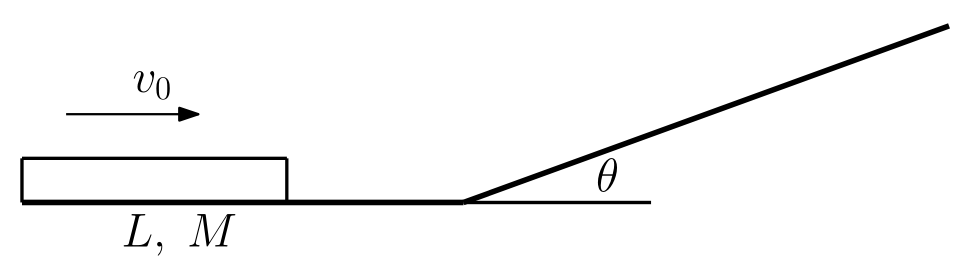
\includegraphics[width=0.7\linewidth]{screenshot001}
			\caption{Trem de comprimento L.}
			\label{fig:fig1}
		\end{figure}

		\part Em termos de quais movimentos é portanto possível descrever o sistema?

		\begin{solution}

		\end{solution}
	\end{parts}



	\question Calcule a expressão para a energia cinética de um sistema de $ N $ corpos no referencial do centro de massa.

	\begin{solution}

	\end{solution}



	\question Considere um trem de comprimento $ L $, massa total $ M $ e densidade uniforme, em movimento com velocidade $ v_0 $ num plano horizontal sem atrito (veja a figura \ref{fig:fig1}). No instante $ t = 0 $, o trem encontra uma subida retilínea que faz um ângulo $ \theta $ em relação ao plano horizontal e começa subir até parar.

	\begin{parts}
		\part Mostre explicitamente que, no cálculo da energia potencial de um corpo não puntiforme, é possível considerar um corpo puntiforme de massa igual à massa total do corpo;

		\begin{solution}

		\end{solution}

		\part \label{part:q5b} Quais as três posições possíveis nas quais o trem pode parar?

		\begin{solution}

		\end{solution}

		\part Calcule a posição do centro de massa do trem quando o trem estiver parado nas três situações do item \ref{part:q5b};

		\begin{solution}

		\end{solution}

		\part Considere agora o caso $ L = \SI{180}{\meter}, M = \SI{200x103}{\kilo\gram}, \theta  = \ang{2} $ e $ v_0 = \SI{180}{\kilo\meter\per\hour} $. Qual a altura final do centro de massa do sistema?

		\begin{solution}

		\end{solution}

		\part Escreva as equações do movimento do trem nas várias fases da subida.

		\begin{solution}

		\end{solution}
	\end{parts}



	\question Considere um foguete que se movimenta na vertical \textit{sob a ação de um campo gravitacional}. Qual a velocidade final do foguete após ter queimado uma parte do combustível? é melhor queimar o combustível rapidamente ou devagar?

	\begin{solution}

	\end{solution}



	\question Um foguete com $ N $ estágios tenta alcançar a velocidade de escape da Terra.

	\begin{figure}[H]
		\centering
		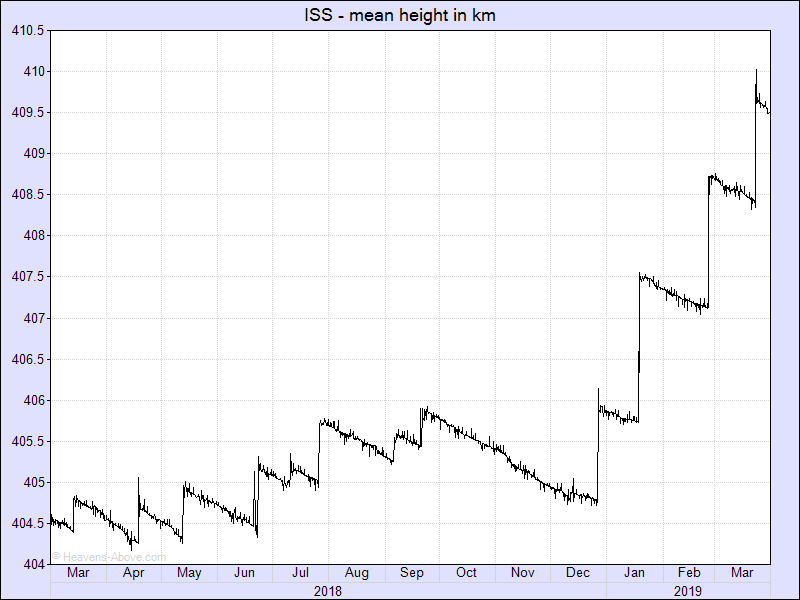
\includegraphics[width=0.7\linewidth]{screenshot002}
		\caption{International Space Station.}
		\label{fig:fig2}
	\end{figure}

	\begin{parts}
		\part Suponha que a razão entre a massa de combustível e a massa de cada um dos tanques seja de 10\%, e que a massa útil represente 1\% da massa total. Qual a velocidade final de um foguete com 3 estágios? E de um foguete com 5 estágios?

		\begin{solution}

		\end{solution}

		\part Para obter velocidades finais maiores \textit{a parte o número de estágios}, é mais eficiente diminuir a massa da carga útil em relação à massa total ou é melhor modificar a razão entre a massa do combustível e a massa dos tanques?

		\begin{solution}

		\end{solution}
	\end{parts}



	\question Num satélite em órbita baixa ao redor da Terra atua uma força de atrito devida à atmosfera do planeta. Essa força de atrito se opõe ao movimento, causando uma diminuição do raio da órbita do satélite. Por exemplo, a Figura \ref{fig:fig2} mostra a altura da \textit{International Space Station} (ISS) em função do tempo, onde podemos claramente identificar os períodos de queda e os períodos (rápidos) onde uma parte do combustível é usada para aumentar a altura. Dado que o atrito é fraco, em cada instante a órbita do satélite é \textit{quase circular}. Relacione a energia cinética à energia potencial do satélite e mostre que (i) a diminuição da energia devido à força de atrito corresponde a uma diminuição da altura da órbita, e (ii) que, apesar da força de atrito estar presente, a velocidade do satélite aumenta com o tempo.

	\begin{solution}

	\end{solution}

	\clearpage

	\question Considere o sistema de polias na figura \ref{fig:fig3}. As mesas que sustentam os corpos $ M_1 $ e $ M_2 $ geram atrito de contato, ambas com coeficiente de atrito $\mu$.

	\begin{figure}[H]
		\centering
		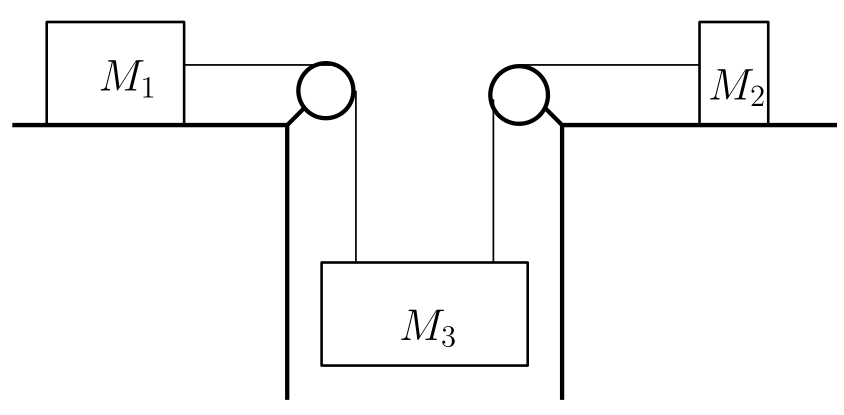
\includegraphics[width=0.7\linewidth]{screenshot003}
		\caption{Sistema de Polias.}
		\label{fig:fig3}
	\end{figure}

	\begin{parts}
		\part Desenhe o diagrama das forças que atuam em cada um dos corpos;

		\begin{solution}
			\centering
			\begin{tikzpicture}
				\newcommand{\tableLen}{3}
				\newcommand{\tableSep}{3}
				\newcommand{\tableDepth}{4}
				\newcommand{\stringH}{0.5}
				\newcommand{\wheelRad}{0.15}
				\draw (0.25,0) rectangle +(1.5,1);

				\draw[thick] (0,0) -- ++(\tableLen,0) -- +(0,-\tableDepth) ($ (\tableLen,0)+(\tableSep,-\tableDepth) $) -- ++(0,\tableDepth) -- +(\tableLen,0);

				\draw (2*\tableLen+\tableSep-0.25,0) rectangle +(-0.8,1);

				\coordinate (aux1) at ($ (\tableLen,0)+(30:\stringH-\wheelRad) $);

				\coordinate (wheelAxis1) at ($ (0,\stringH-|aux1)+(0,-\wheelRad) $);

				\coordinate (aux2) at ($ (\tableLen+\tableSep,0)+(30:-\stringH+\wheelRad) $);

				\coordinate (wheelAxis2) at ($ (0,\stringH-|aux2)+(0,-\wheelRad) $);


				\draw[thick] let \p1=($ (wheelAxis1)+(\wheelRad,0) $) in (1.75,\stringH) -- (0,\stringH-|wheelAxis1) arc (90:0:\wheelRad) -- (\x1,-2) coordinate (string1);

				\draw[thick] let \p1=($ (wheelAxis2)+(-\wheelRad,0) $) in (2*\tableLen+\tableSep-1.05,\stringH) -- (0,\stringH-|wheelAxis2) arc (90:180:\wheelRad) -- (\x1,-2) coordinate (string2) (\tableLen+\tableSep-0.2,-2) rectangle +(-\tableSep+0.4,-0.8);

				\draw (\tableLen,0) -- (wheelAxis1) circle (\wheelRad)
				(\tableLen+\tableSep,0) -- (wheelAxis2) circle (\wheelRad);

				\node at (\tableLen+0.5*\tableSep,-2.4) {\large $ M_3 $};
				\node at (1,0.5) {\large $ M_1 $};
				\node at (2*\tableLen+\tableSep-0.25-0.4,0.5) {\large $ M_2 $};

				\draw[-Latex] (\tableLen+0.5*\tableSep,-2.8) -- node[right] {$ \vec{P_3} $} +(0,-1);
				\draw[-Latex] (string1) -- node[right] {$ \vec{T_1'} $} +(0,0.8);
				\draw[-Latex] (string2) -- node[left] {$ \vec{T_2'} $} +(0,1);

				\draw[-Latex] (0.25+1.5,0.5) -- node[above] {$ \vec{T_1} $} +(0.8,0);

				\draw[-Latex] (0.25,0.5) -- node[above] {$ \vec{F_{at\,1}} $} +(-1,0);

				\draw[-Latex] (2*\tableLen+\tableSep-0.25-0.8,0.5) -- node[above] {$ \vec{T_2} $} +(-1,0);
				\draw[-Latex] (2*\tableLen+\tableSep-0.25,0.5) -- node[above] {$ \vec{F_{at\,2}} $} +(1.2,0);

				\draw[-Latex] (1,0) -- node[right] {$ \vec{P_1} $} +(0,-1);
				\draw[-Latex] (2*\tableLen+\tableSep-0.25-0.4,0) -- node[right] {$ \vec{P_2} $} +(0,-1.2);

				\draw[-Latex] (1,1) -- node[right] {$ \vec{N_1} $} +(0,1);
				\draw[-Latex] (2*\tableLen+\tableSep-0.25-0.4,1) -- node[right] { $ \vec{N_2} $} +(0,1.2);
			\end{tikzpicture}
		\end{solution}

		\part Como você pode escrever de forma matemática o vínculo entre os corpos devido às cordas?

		\begin{solution}
			Somando as forças em cada corpo, encontramos as expressões para a força resultante:
			\begin{align}
				\vec{F_{r\,1}} & =\vec{P_{1}}+\vec{N_1}+\vec{T_1}+\vec{F_{at\,1}}\label{eq:Fr1} \\
				\vec{F_{r\,2}} & =\vec{P_{2}}+\vec{N_2}+\vec{T_2}+\vec{F_{at\,2}}\label{eq:Fr2} \\
				\vec{F_{r\,3}} & =\vec{P_{3}}+\vec{T_1'}+\vec{T_2'}\label{eq:Fr3}
			\end{align}
			Assumindo que as polias transferem o movimento e as forças perfeitamente, pela terceira lei de Newton, temos que $ \vec{T_1}=-\vec{T_1'} $ e $ \vec{T_2}=-\vec{T_2'} $, portanto, por \ref{eq:Fr1}, \ref{eq:Fr2} e \ref{eq:Fr3}, temos:
			\begin{gather*}
				\left\lbrace
				\begin{aligned}
					\vec{T_1} & =\vec{F_{r\,1}}-\del{\vec{P_{1}}+\vec{N_1}+\vec{F_{at\,1}}}\nonumber \\
					\vec{T_2} & =\vec{F_{r\,2}}-\del{\vec{P_{2}}+\vec{N_2}+\vec{F_{at\,2}}}
				\end{aligned}\right. \implies\nonumber\\
				\vec{F_{r\,3}}=\vec{P_{3}}+\del{\vec{P_{1}}+\vec{N_1}+\vec{F_{at\,1}}}-\vec{F_{r\,1}}+\del{\vec{P_{2}}+\vec{N_2}+\vec{F_{at\,2}}}-\vec{F_{r\,2}}
			\end{gather*}
			assumindo que os planos são horizontais, os pesos se cancelam com as forças normais, e ficamos com
			\[ \vec{F_{r\,3}}=\vec{P_{3}}+\vec{F_{at\,1}}-\vec{F_{r\,1}}+\vec{F_{at\,2}}-\vec{F_{r\,2}} \]
			Sendo $ \vec{a_i} $ a aceleração de um corpo $ i $, pela segunda lei de Newton, temos:
			\begin{equation}\label{eq:Fr3rep}
				\begin{aligned}
					M_3\,\vec{a_3}=M_3\,\vec{g}+\vec{F_{at\,1}}-M_1\,\vec{a_1}+\vec{F_{at\,1}}-M_2\,\vec{a_2} & \implies \\
					M_1\,\vec{a_1}-\vec{F_{at\,1}}+M_2\,\vec{a_2}-\vec{F_{at\,1}}+M_3\del{\vec{a_3}-\vec{g}}  & =0
				\end{aligned}
			\end{equation}

			\paragraph{Nota:}
			Perceba que não podemos escrever $\vec{F_{at\,i}}=-\mu\,\vec{N_i}$ e nem $\vec{F_{at\,i}}=-\mu\,N_i\,\ihat$, pois \textbf{não há} eixos definidos em nossa resolução\footnote{Note, porém, que é possível escrever $ \vec{F_{at\,i}}=-\mu\,N_i\,\dot{\hat{r}} $, onde $ \hat{r} $ é o vetor unitário do deslocamento (\href{https://physics.stackexchange.com/questions/77458/about-vector-form-of-friction}{fonte}).}.
		\end{solution}

		\part Escreva as equações do movimento para cada um dos corpos.

		\begin{solution}
			Sejam $ (x_1,0) $ as coordenadas do centro de massa do corpo 1, tomadas a partir do canto superior da polia esquerda, com o eixo $ x_1 $ positivo para a esquerda, $ (x_2,0) $ as coordenadas do centro de massa do corpo 2, tomadas a partir do canto superior da polia direita, com o eixo $ x_2 $ positivo para a direita, e $ (0,y) $ as coordenadas do centro de massa do corpo 3, tomadas a partir do centro do diagrama.

			\medskip

			\begin{multi}

				\begin{center}
					\begin{tikzpicture}[scale=0.8]
						\newcommand{\tableLen}{3}
						\newcommand{\tableSep}{3}
						\newcommand{\tableDepth}{4}
						\newcommand{\stringH}{0.5}
						\newcommand{\wheelRad}{0.15}
						\draw (0.25,0) rectangle +(1.5,1);

						\draw[thick] (0,0) -- ++(\tableLen,0) -- +(0,-\tableDepth) ($ (\tableLen,0)+(\tableSep,-\tableDepth) $) -- ++(0,\tableDepth) -- +(\tableLen,0);

						\draw (2*\tableLen+\tableSep-0.25,0) rectangle +(-0.8,1);

						\coordinate (aux1) at ($ (\tableLen,0)+(30:\stringH-\wheelRad) $);

						\coordinate (wheelAxis1) at ($ (0,\stringH-|aux1)+(0,-\wheelRad) $);

						\coordinate (aux2) at ($ (\tableLen+\tableSep,0)+(30:-\stringH+\wheelRad) $);

						\coordinate (wheelAxis2) at ($ (0,\stringH-|aux2)+(0,-\wheelRad) $);


						\draw[thick] let \p1=($ (wheelAxis1)+(\wheelRad,0) $) in (1.75,\stringH) -- (0,\stringH-|wheelAxis1) arc (90:0:\wheelRad) -- (\x1,-2) coordinate (string1);

						\draw[thick] let \p1=($ (wheelAxis2)+(-\wheelRad,0) $) in (2*\tableLen+\tableSep-1.05,\stringH) -- (0,\stringH-|wheelAxis2) arc (90:180:\wheelRad) -- (\x1,-2) coordinate (string2) (\tableLen+\tableSep-0.2,-2) rectangle +(-\tableSep+0.4,-0.8);

						\draw (\tableLen,0) -- (wheelAxis1) circle (\wheelRad)
						(\tableLen+\tableSep,0) -- (wheelAxis2) circle (\wheelRad);

						\node at (\tableLen+0.5*\tableSep,-2.4) {$ (0,y) $};
						\node at (1,0.5) {$ (x_1,0) $};
						\draw[<-] (2*\tableLen+\tableSep-0.25-0.4,0.5) -- +(1,0) node[right] {$ (x_2,0) $};

						\draw[->] (\tableLen-0.5,-0.2) -- +(0,-1) node[below] {$ y $};
						\draw[->] (\tableLen+\tableSep+0.5,-0.2) -- +(0,-1) node[below] {$ y $};

						\draw[->] (\tableLen-0.2,-0.5) -- +(-1,0) node[left] {$ x_1 $};
						\draw[->] (\tableLen+\tableSep+0.2,-0.5) -- +(1,0) node[right] {$ x_2 $};
					\end{tikzpicture}
				\end{center}
				\nextcol

				Esse centro pode ser tido como a intercessão das duas polias, num diagrama simplificado utilizando os centros de massa, somente.

				\begin{center}
					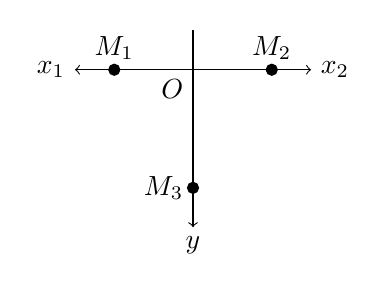
\begin{tikzpicture}
						\draw[->] (0,0) node[below left] {$ O $} -- (1.5,0) node[right] {$ x_2 $};
						\draw[->] (0,0) -- (-1.5,0) node[left] {$ x_1 $};
						\draw[->] (0,0.5) -- (0,-2) node[below] {$ y $};

						\filldraw (-1,0) circle (2pt) node[above] {$ M_1 $};

						\filldraw (1,0) circle (2pt) node[above] {$ M_2 $};

						\filldraw (0,-1.5) circle (2pt) node[left] {$ M_3 $};
					\end{tikzpicture}
				\end{center}
			\end{multi}

			Tomando as mesmas suposições do item anterior, por \ref{eq:Fr1}, \ref{eq:Fr2} e \ref{eq:Fr3}, temos:
			\begin{align}
				\vec{F_{r\,1}} & =\vec{T_1}+\vec{F_{at\,1}}\label{eq:Fr1red}           \\
				\vec{F_{r\,2}} & =\vec{T_2}+\vec{F_{at\,2}}\label{eq:Fr2red}           \\
				\vec{F_{r\,3}} & =\vec{P_3}-\del{\vec{T_1}+\vec{T_2}}\label{eq:Fr3red}
			\end{align}
			Sendo $ \vec{r_i} $ o vetor posição de um corpo $ i $, pela segunda lei de Newton, temos:
			\begin{align}
				M_1\,\ddot{\vec{r}}_{\mathbf{1}} & =\vec{T_1}+\vec{F_{at\,1}}\label{eq:Motion1}           \\
				M_2\,\ddot{\vec{r}}_{\mathbf{2}} & =\vec{T_2}+\vec{F_{at\,2}}\label{eq:Motion2}           \\
				M_3\,\ddot{\vec{r}}_{\mathbf{3}} & =\vec{P_3}-\del{\vec{T_1}+\vec{T_2}}\label{eq:Motion3}
			\end{align}

			%			Como $ \vec{T_1} $ e $\vec{T_2}$ só dependem da massa $M_3$, podemos concluir que ambos corpos 1 e 2 serão puxados para o centro, enquanto o corpo 3 cai, supondo que o atrito seja cinético (o que implica que todos os corpos estão em movimento).

			Adotemos a notação $ |\vec{v}|=v $.

			Como os corpos 1 e 2 tem seu movimento restrito à horizontal, e o corpo 3 tem seu movimento somente na vertical, de \ref{eq:Motion1}, \ref{eq:Motion2} e \ref{eq:Motion3}, % tomando $ |\vec{F_{at\,i}}|=\mu\,M_i\,g $ para um corpo $ i $,
			temos:
			\begin{align}
				M_1\,\ddot{x}_1 & =-T_1+F_{at\,1}\label{eq:mov1}    \\
				M_2\,\ddot{x}_2 & =-T_2+F_{at\,2}\label{eq:mov2}    \\
				M_3\,\ddot{y}   & =P_3-\del{T_1+T_2}\label{eq:mov3}
			\end{align}
			\paragraph{Nota:}
			Apesar de $ \vec{T_1'} $ e $\vec{T_2'}$ estarem opostos a trajetória do corpo 3, seguindo o princípio de que em cada ponto de uma corda ideal temos a mesma tensão em cada lado, podemos ver que $ \vec{T_1} $ e $ \vec{T_2} $ estão apontando no sentido positivo do eixo $ y $:

			\medskip

			\begin{multi}[3]
				\centering
				\begin{tikzpicture}
					\newcommand{\tableLen}{3}
					\newcommand{\tableSep}{3}
					\newcommand{\tableDepth}{4}
					\newcommand{\stringH}{0.5}
					\newcommand{\wheelRad}{0.15}

					\clip (\tableLen+0.5*\tableSep,-2.9) rectangle (2*\tableLen+\tableSep,1);

					\draw[thick] ($ (\tableLen,0)+(\tableSep,-\tableDepth) $) -- ++(0,\tableDepth) -- +(\tableLen,0);

					\draw (2*\tableLen+\tableSep-0.25,0) rectangle +(-0.8,1);

					\coordinate (aux2) at ($ (\tableLen+\tableSep,0)+(30:-\stringH+\wheelRad) $);

					\coordinate (wheelAxis2) at ($ (0,\stringH-|aux2)+(0,-\wheelRad) $);

					\draw[thick] let \p1=($ (wheelAxis2)+(-\wheelRad,0) $) in (2*\tableLen+\tableSep-1.05,\stringH) -- (0,\stringH-|wheelAxis2) arc (90:180:\wheelRad) -- (\x1,-2) coordinate (string2) (\tableLen+\tableSep-0.2,-2) rectangle +(-\tableSep+0.4,-0.8);

					\draw (\tableLen+\tableSep,0) -- (wheelAxis2) circle (\wheelRad);

					\node at (\tableLen+0.7*\tableSep,-2.4) {\large $ M_3 $};
					\node at (2*\tableLen+\tableSep-0.25-0.4,0.5) {\large $ M_2 $};

					\draw[-Latex,red,thick] (2*\tableLen+\tableSep-0.25-0.8,0.5) -- node[above] {$ \vec{T_2} $} +(-1,0);
				\end{tikzpicture}

				\nextcol

				\centering
				\begin{tikzpicture}
					\newcommand{\tableLen}{3}
					\newcommand{\tableSep}{3}
					\newcommand{\tableDepth}{4}
					\newcommand{\stringH}{0.5}
					\newcommand{\wheelRad}{0.15}

					\clip (\tableLen+0.5*\tableSep,-2.9) rectangle (2*\tableLen+\tableSep,1);

					\draw[thick] ($ (\tableLen,0)+(\tableSep,-\tableDepth) $) -- ++(0,\tableDepth) -- +(\tableLen,0);

					\draw (2*\tableLen+\tableSep-0.25,0) rectangle +(-0.8,1);

					\coordinate (aux2) at ($ (\tableLen+\tableSep,0)+(30:-\stringH+\wheelRad) $);

					\coordinate (wheelAxis2) at ($ (0,\stringH-|aux2)+(0,-\wheelRad) $);

					\draw[thick] let \p1=($ (wheelAxis2)+(-\wheelRad,0) $) in (2*\tableLen+\tableSep-1.05,\stringH) -- (0,\stringH-|wheelAxis2) arc (90:180:\wheelRad) -- (\x1,-2) coordinate (string2) (\tableLen+\tableSep-0.2,-2) rectangle +(-\tableSep+0.4,-0.8);

					\draw (\tableLen+\tableSep,0) -- (wheelAxis2) circle (\wheelRad);

					\node at (\tableLen+0.7*\tableSep,-2.4) {\large $ M_3 $};
					\node at (2*\tableLen+\tableSep-0.25-0.4,0.5) {\large $ M_2 $};

					\draw[-Latex,red,thick] let \p1=(aux2) in (\x1,0.5) -- node[above] {$ \vec{T_2} $} +(-1,0);
				\end{tikzpicture}

				\nextcol

				\centering
				\begin{tikzpicture}
					\newcommand{\tableLen}{3}
					\newcommand{\tableSep}{3}
					\newcommand{\tableDepth}{4}
					\newcommand{\stringH}{0.5}
					\newcommand{\wheelRad}{0.15}

					\clip (\tableLen+0.5*\tableSep,-2.9) rectangle (2*\tableLen+\tableSep,1);

					\draw[thick] ($ (\tableLen,0)+(\tableSep,-\tableDepth) $) -- ++(0,\tableDepth) -- +(\tableLen,0);

					\draw (2*\tableLen+\tableSep-0.25,0) rectangle +(-0.8,1);

					\coordinate (aux2) at ($ (\tableLen+\tableSep,0)+(30:-\stringH+\wheelRad) $);

					\coordinate (wheelAxis2) at ($ (0,\stringH-|aux2)+(0,-\wheelRad) $);

					\draw[thick] let \p1=($ (wheelAxis2)+(-\wheelRad,0) $) in (2*\tableLen+\tableSep-1.05,\stringH) -- (0,\stringH-|wheelAxis2) arc (90:180:\wheelRad) -- (\x1,-2) coordinate (string2) (\tableLen+\tableSep-0.2,-2) rectangle +(-\tableSep+0.4,-0.8);

					\draw (\tableLen+\tableSep,0) -- (wheelAxis2) circle (\wheelRad);

					\node at (\tableLen+0.7*\tableSep,-2.4) {\large $ M_3 $};
					\node at (2*\tableLen+\tableSep-0.25-0.4,0.5) {\large $ M_2 $};

					\draw[-Latex,red,thick] ($ (string2)+(0,2) $) -- node[left] {$ \vec{T_2} $} +(0,-1);
				\end{tikzpicture}
			\end{multi}

			Sendo o comprimento das cordas constante, igual a $ \ell_1 $ para a corda entre 1 e 3, e igual a $ \ell_2 $ para a corda entre 2 e 3, temos:
			\begin{align}
				\ell_1 & =x_1+y\implies & \ddot{x}_1+\ddot{y} & =0\implies & \ddot{y} & =-\ddot{x}_1\label{eq:ddotyx1} \\
				\ell_2 & =x_2+y\implies & \ddot{x}_2+\ddot{y} & =0\implies & \ddot{y} & =-\ddot{x}_2\label{eq:ddotyx2}
			\end{align}
			Seja a força total $ \vec{F_{r\,t}}=\vec{F_{r\,1}}+\vec{F_{r\,2}}+\vec{F_{r\,3}} $, por \ref{eq:Fr1red}, \ref{eq:Fr2red} e \ref{eq:Fr3red}, temos:
			\begin{align}
				|\vec{F_{r\,t}}|=|\vec{F_{r\,1}}|+|\vec{F_{r\,2}}|+|\vec{F_{r\,3}}| & =|\vec{T_1}+\vec{F_{at\,1}}|+|\vec{T_2}+\vec{F_{at\,2}}|+|\vec{P_3}-\del{\vec{T_1}+\vec{T_2}}| \\
				\intertext{substituindo \ref{eq:mov1}, \ref{eq:mov2}, \ref{eq:mov3}}
				M_3\,\ddot{y}-M_1\,\ddot{x}_1-M_2\,\ddot{x}_2                       & =P_3-\del{T_1+T_2}-\del{-T_1+F_{at\,1}}-\del{-T_2+F_{at\,2}}\nonumber                          \\
				\intertext{substituindo \ref{eq:ddotyx1} e \ref{eq:ddotyx2}}
				\del{M_1+M_2+M_3}\ddot{y}                                           & =P_3-\del{F_{at\,1}+F_{at\,2}}=F_{r\,t}\label{eq:FmaFinal}
				%			\intertext{sendo a massa total do sistema $ M_t=M_1+M_2+M_3 $, pela segunda lei de Newton, do lado esquerdo temos a força total resultante no sistema, $ F_{r\,t} $:}
				%				F_{r\,t}&=P_3-\del{F_{at\,1}+F_{at\,2}}
			\end{align}
		\end{solution}

		\part A energia é conservada no sistema?

		\begin{solution}
			Não, pois há ação de forças dissipativas, nomeadamente, o atrito entre os corpos e a superfície.
		\end{solution}

		\part Considerando o sistema $ M_1 + M_2 + M_3 $, o momento linear é conservado? Por quê?

		\begin{solution}
			Sendo $ \vec{F}=\dod{\vec{p}}{t} $, para o caso em que $ \vec{F}=\vec{0} $, o momento linear do sistema é conservado, já que uma derivada nula implica que a quantidade é constante.

			Analisando \ref{eq:FmaFinal}, podemos ver que essa expressão só é nula para $ P_3=F_{at\,1}+F_{at\,2} $, portanto, o momento linear não é conservado no caso geral.

			De forma genérica, podemos dizer que, como há forças externas atuando no sistema, o momento linear não é conservado.

			\paragraph{Nota:}
			O momento linear seria conservado caso incluíssemos as superfícies em nossa análise, já que o atrito é resultado da interação entre os blocos e as superfícies\footnote{Fonte: \url{https://physics.stackexchange.com/questions/79884/conservation-of-momentum-when-friction-is-present}.}.
		\end{solution}
	\end{parts}

	\clearpage

	\question Um caminhão-tanque cheio de água, de massa total $ M $, utilizado para limpar ruas com um jato de água, trafega por uma via horizontal, com coeficiente de atrito cinético $\mu$. Ao atingir a velocidade $ v_0 $, o motorista coloca a marcha no ponto morto e liga o jato de água, que é enviada para trás com velocidade ve relativa ao caminhão, com uma vazão de $ \lambda $ litros por segundo. Ache a velocidade $ v(t) $ do caminhão depois de um tempo $ t $.

	\begin{solution}

	\end{solution}

\end{questions}
\end{document}
